\documentclass{article}

\usepackage{multirow}
\usepackage{booktabs}
\usepackage{tabularx}
\usepackage{graphicx}
\usepackage{float}
\usepackage{hyperref}
\usepackage{enumitem}
\hypersetup{
    colorlinks,
    citecolor=black,
    filecolor=black,
    linkcolor=red,
    urlcolor=blue
}

% ================ Commands ===============

\newcounter{acnum}
\newcommand{\actheacnum}{AC\theacnum}
\newcommand{\acref}[1]{AC\ref{#1}}
\newcounter{ucnum}
\newcommand{\uctheucnum}{UC\theucnum}
\newcommand{\uref}[1]{UC\ref{#1}}
\newcounter{mnum}
\newcommand{\mthemnum}{M\themnum}
\newcommand{\mref}[1]{M\ref{#1}}

% ================ Title ===============

\title{
    \vspace{40mm}
	\textbf {
	\Huge {\color[rgb]{0.9,0,0}Blaze} Brigade \\
	\large - Module Guide -}}

\date{\today}

\author{SFWR ENG 3XA3 - Section L02 \\
	007 (Group 7) \\ \\
	Jeremy Klotz - klotzjj \\
	Asad Mansoor - mansoa2 \\
	Thien Trandinh - trandit \\
	Susan Yuen - yuens2}
	
% =============== Document ===============
	
\begin{document}

\maketitle
\pagenumbering{gobble}
\newpage
\pagenumbering{arabic}

\tableofcontents
\listoftables
\listoffigures

\newpage 
\begin{table}[bp]
    \caption{\bf Revision History}
    \begin{tabularx}{\textwidth}{p{3cm}p{2cm}X}
        \toprule {\bf Date} & {\bf Version} & {\bf Notes} \\
        \midrule
        Nov 13, 2016 & 1.0 & Completed Design Document \\
        Dec 07, 2016 & 2.0 & Revised section 3-7 with the modification of new modules \\
        \bottomrule
    \end{tabularx}
\end{table}
 
\hfill \break

% =============== Section 1 ===============

\newpage

\section{Introduction}

\subsection{Summary of Project}
Blaze Brigade is a tactical simulation role-playing game that combines the strategic challenges as a form of interactive entertainment for its users. This turn-based game allows users to advance their units into enemy territory, participate in combat, and strive to eliminate all of the opposing units. In adaption to the open-source freeware, Tactics Heroes, Blaze Brigade will incorporate new functional and design enhancements that may not be available on the existing open-source project. Such enhancements include the implementation of new features within the unit movement, combat and strategy aspects of the game as well as improved graphical representations of the main menu and gameplay to improve the overall experience of the game.

\subsection{Context of Module Guide}
The system is fully devised and presents all of its functional and non-functional requirements in the Software Requirements Specification (SRS), stating desirable properties of the system. Meanwhile, the Design Document will further evaluate on how these requirements are identified and achieved. The Module Guide (MG) will serve as a tool to decompose the following system into a modular structure, adhering to the principle of information hiding. Upon reaching the finalized version of this document, the Module Guide can be distributed amongst various groups in order to learn and identify parts of the software that is being presented. These various groups are as follows:

\begin{itemize}
    \item \textbf{Developers and Maintenance:} System decomposition and the Module Guide will aid the developers and maintenance team in understanding the system-as-is and to recognize which areas of the software are likely to be changed. In addition, a sense of the overall design will be structured and will be maintained in the following developments phases yet to come.
    \item \textbf{Designers:} In addition to the design pattern being documented, designers are able to determine whether the designs are constructed as initially specified. Along with the upcoming anticipated changes to be happening, designers can further determine which areas of software are flexible and feasible to accommodate new design changes.
    \item \textbf{New Recruits or Outsourced Resources:} The documentation will aid with the onboarding process of new recruits in familiarizing the overall structure of the implementation adhering to a specific design principle. This will reduce the downtime of debugging and have an advantage of multiple groups working on the system simultaneously. Furthermore, if an external team were to implement the system or would like to carry out further improvements after the project timeline, this document will serve as an aid to determine the existing framework and how further implementation can take place.
\end{itemize}

\noindent
In addition to the Module Guide, the Module Interface Specification (MIS) is also a product of the design documentation. The specification defines the syntax and semantics that are associated with the functions provided in the source code. Tools like Doxygen have been utilized to generate a set of documentation that will indicate the characteristics of the functions in terms of the corresponding inputs, outputs, assumptions, exceptions, state and environment variables. These characteristics will further aid in observing how the implementation has taken place and how the design constitutes from these functions.

\subsection{Design Principle}
The design principle taken into consideration revolves around the decomposition of the overall system into a modular structure of subsystems. These subsystems are observed in an abstract manner, hiding any details that may complicate the process. This act of information hiding and encapsulation ensures that each module hides some design aspect from the rest of the system and analyzes which areas are expected to change. Hence, this document follows a design for change pattern and will be in the best interest throughout all of the subsystems presented in the system. For instance, the anticipated changes within the system would have been encapsulated in this process to ensure that any further changes to the design does not disrupt the main design interface of the system. As a principle for the decomposition into modular structure, the instance of low coupling is desired as the result is given as independent modules. In the same respect, high cohesion within the modules is highly desired since the elements of each module are strongly related to the module's characteristics. Therefore, this process is motivated around the concept of design for change as an exercise and validation to protect other modules of the system if any major changes occur in the overall design.

\subsection{Outline of Module Guide}
The Module Guide is organized in the given order. Section \ref{SecChange} lists all of the anticipated and unlikely changes that the software system might contain. Section \ref{SecMH} decomposes the system into a list of modules, and further states the module hierarchy. Section \ref{SecConnection} establishes the connection between the software requirements with the modules. Section \ref{SecMD} gives a detailed insight on how the modules have been decomposed with their corresponding descriptions. Section \ref{SecTM} includes three traceability matrices comparing the modules with the software requirements and anticipated changes as referenced earlier in Section \ref{SecConnection}. At last, section \ref{SecUse} pinpoints the use hierarchy between the modules initialized to establish connection between the independent modules.

\subsection{Definitions, Acronyms, Abbreviations, Symbols}
The following definitions and symbols are defined in Table \ref{TblDFN} and will be referenced throughout the remainder of the Module Guide.
\begin{table}[H]
    \centering
    \begin{tabular}{p{2cm} p{8.5cm}}
        \toprule
        \textbf{Symbol} & \textbf{Description} \\
        \midrule
        SRS & Software Requirements Specification document \\
        MG  & Module Guide document \\
        MIS & Module Interface Specification document \\
        Module & A decomposed subsystem of the overall software system \\
        AC & Anticipated Changes \\
        UC & Unlikely Changes \\
        MVC & Model-View-Controller \\
        FR & Functional Requirements \\
        NFR & Non-Functional Requirements \\
        \bottomrule
    \end{tabular}
    \caption{List of Definitions, Acronyms, Abbreviations and Symbols}
    \label{TblDFN}
\end{table}

% =============== Section 2 ===============

\section{Anticipated and Unlikely Changes} \label{SecChange}

\subsection{Anticipated Changes} \label{SecAchange}
The design decisions in this section are categorized as anticipated due to being hidden in modules. When these changes are made, they can be done easily and will not affect other modules of the project.

\begin{description}[leftmargin=1.2cm]
    \item[\refstepcounter{acnum} \actheacnum \label{acClass}:] All classes that implement the Class interface are likely to have their stats change for balancing reasons.
    \item[\refstepcounter{acnum} \actheacnum \label{acWeapon}:] All weapons that implement the Weapon interface are likely to have their stats change for balancing reasons.
    \item[\refstepcounter{acnum} \actheacnum \label{acDamageCalculations}:] The getHitRate() and getCritRate() methods inside the DamageCalculations class are likely to change for balancing reasons.
    \item[\refstepcounter{acnum} \actheacnum \label{acSprites}:] All sprites from outside sources are likely to change. It has been determined that the project should contain all original content.
\end{description}

\subsection{Unlikely Changes} \label{SecUchange}
The following design decisions are unlikely to change because they affect many modules. Since they affect multiple modules, changing these decisions may result in multiple changes in the overall design of the project. Unless these changes are necessary, they will not occur.

\begin{description}[leftmargin=1.2cm]
    \item[\refstepcounter{ucnum} \uctheucnum \label{ucIO}:] Input/Output devices
      (Input: Mouse, Output: Updated Model and Screen).
    \item[\refstepcounter{ucnum} \uctheucnum \label{ucArchitecture}:] The software implements the MVC (Model-View-Controller) architecture.
    \item[\refstepcounter{ucnum} \uctheucnum \label{ucGraph}:] The Graph of nodes that represents the playable grid.
    \item[\refstepcounter{ucnum} \uctheucnum \label{ucNodeIdentification}:] Nodes are identified by their x and y coordinates.
    \item[\refstepcounter{ucnum} \uctheucnum \label{ucPathfinder}:] The path finding algorithm.
\end{description}

% =============== Section 3 ===============

\section{Module Hierarchy} \label{SecMH}

\begin{description}
    \item [\refstepcounter{mnum} \mthemnum \label{HHm}:] Hardware-Hiding Module
    \item [\refstepcounter{mnum} \mthemnum \label{Mm}:] Model Module
    \item [\refstepcounter{mnum} \mthemnum \label{Vm}:] View Module
    \item [\refstepcounter{mnum} \mthemnum \label{Cm}:] Controller Module
\end{description}

\begin{table}[H]
    \centering
    \begin{tabular}{p{0.25\textwidth} p{0.6\textwidth}}
        \toprule
        \textbf{Level 1} & \textbf{Level 2} \\
        \midrule
        Hardware-Hiding Module & C\# XNA Game Studio \\
        Model Module  & Map Module, Unit Module, Weapon Module, Game State, Player \\
        View Module & Menu Module, Animation, Camera, DrawClass, Sound \\
        Controller Module & Game, GameFunction, MouseHandler, Damage Calculation\\
        \bottomrule
    \end{tabular}
    \caption{Module Hierarchy}
    \label{TblMH}
\end{table}

% =============== Section 4 ===============

\section{Connection Between Requirements and Design} \label{SecConnection}

The system is intended to satisfy all of the functional and non-functional requirements that were initially specified in the SRS. In this section, the system is decomposed into modules and connections are assessed between the decomposed requirements with the corresponding requirements. These are shown in the Table \ref{TblRT} and Table \ref{TblNFRT} under Section \ref{SecTM}. \\

All the requirements can be categorized as one of the modules provided in the Module Hierachy. For instance, the Menu Model extends through all of the requirements that initiate the menu option in one way or another. The model module encapsulates the model classes that represent the structure of the source code. The View module is primarily what users get to see as a final product, including the various parameters within the game. Finally, all game logic is handled inside the Controller module. One such example to prove the above would be appearance requirements. Appearance requirements specify the look and feel that the user should be expecting from the product and heavily focuses on the view module. These modules initialized will cover those aspects and model this case scenario in such a manner that each module or sub-module will be independent and protected if there is design change in the other part of the system.

% =============== Section 5 ===============

\section{Module Decomposition} \label{SecMD}

The goal of this section is to provide a detailed description of how the system operates. In order to do this, a module decomposition is necessary. The modules in this decomposition are not classes directly from the software code, but instead are a collection of sub-modules that complete an abstract concept. The sub-modules may be classes directly from the software, or be broken down until these classes are reached. This section will also include a pair of diagrams, one that explains the project's chosen architecture, and another that demonstrates how each module fits into said architecture. 

\subsection{System Architecture}

The following definitions explain all important terms used to describe the system architecture.

\begin{description}[leftmargin=0.2cm]
    \item \textbf{MVC $\rightarrow$} The specific system architecture for this software. MVC stands for Model-View-Controller. The user interacts with the controller, which manipulates the model. The view then updates based on the model. From here, the user sees the result of their interaction through the view.
    \item \textbf{Model $\rightarrow$} The central point of the system architecture. The model contains all data, logic and rules of the software. Whatever the view displays to the user is based on the model.
    \item \textbf{View $\rightarrow$} The part of the system that displays information to the user. This is where the user sees all relevant information.
    \item \textbf{Controller $\rightarrow$} The part of the system that the user manipulates. The controller is what updates all information stored in the model.
    \begin{figure}[H]
        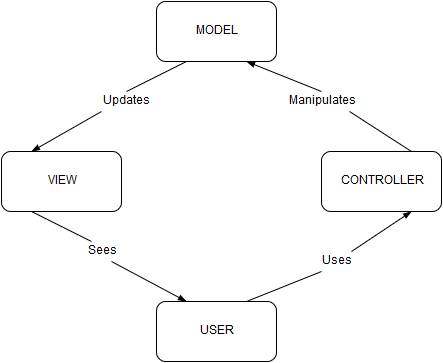
\includegraphics[width=\textwidth]{SystemArchitecture.png}
        \caption{The MVC Architecture of the Software System}
    \end{figure}
\end{description}

\subsection{Underlaying Architecture}

Now that the general idea of the system has been explained, this section will take the level of abstraction one step further. This level of abstraction demonstrates the module decomposition of the system. Arrows in the diagram represent sub-modules that help reach the next module in the system. Note that this is not a uses diagram, nor is it intended to be.

\begin{description}[leftmargin=0.2cm]
    \item \textbf{Hardware Hiding Module:} This module consists of C\# XNA Game Studio, and provides an interface for users to interact with the software. This module will convert the raw input data from the mouse into data that can be used by the controller to update the current game state. The view will also be implemented through this, allowing for users to correctly interact with the software.
    \item \textbf{Model Module:} This model contains the structure of the game. Most of the elements in this module are simply data such as unit stats and position. The majority of the methods in this module are simple C\# properties (special C\# method that functions as both a getter and setter).
    \item \textbf{View Module:} This module contains all view related features. This module displays data to the users in the form of graphics representing the current game state.
    \item \textbf{Controller Module:} This module handles all the software decision making of Blaze Brigade, including how the entirety of the game functions as a whole. This includes all visible behavior of the system specified in the SRS. Hence, any changes to the SRS will hereby result in modifications to this module.
    
\end{description}

\subsection{Leaf-level Decomposition}
Another level of decomposition is yet required for Blaze Brigade. This will include the decomposition of the smaller modules listed in section 3 that are a grouped under model, view and controller modules. 

\subsubsection{Map Module}
This module is further broken down into Graph and Node.

\begin{itemize}
    \item \textbf{Graph:} This is the graph structure used to represent the game map grid and is comprised of Nodes. 
    \item \textbf{Node:} The structure that represents each tile on the game map grid.
\end{itemize}

\subsubsection{Unit Module}
This module is further broken down into Warrior, Mage and Archer.

\begin{itemize}
    \item \textbf{Warrior:} One of the 3 playable unit classes with high physical attack and defense.
    \item \textbf{Archer:} One of the 3 playable unit classes with high skill and speed.
    \item \textbf{Mage:} One of the 3 playable unit classes with high magical attack and defense.
\end{itemize}

\subsubsection{Weapon Module}
This module is further broken down into Bronze Sword, Iron Sword, Short Bow, Long Bow, Fireball, and Fireblast.
\begin{itemize}
    \item \textbf{Bronze Sword:} A warrior's weapon.
    \item \textbf{Iron Sword:} A warrior's weapon.
    \item \textbf{Short Bow:} An archer's weapon.
    \item \textbf{Long Bow:} An archer's weapon.
    \item \textbf{Fireball:} A mage's weapon.
    \item \textbf{Fireblast:} A mage's weapon.
\end{itemize}

\subsubsection{Menu Module}
The GUI module is further broken down into Main Menu, HowToPlay, HowToPlay2, and HowToPlay3.
\begin{itemize}
    \item \textbf{Main Menu:} The Main menu upon start-up that allows for navigation to the rest of the game.
    \item \textbf{HowToPlay:} The first page of instructions on how to play.
    \item \textbf{HowToPlay2:} The second page of instructions on how to play.
    \item \textbf{HowToPlay3:} The third page of instructions on how to play.
\end{itemize}

\subsection{Summary of Leaf Modules}

Unit Module and Weapon Module are treated as the smallest decomposition to a leaf module for convenience as every unit in Unit Module and every weapon in Weapon module are almost identical outside of game parameters such as movement and damage dealt. HowToPlay, HowToPlay2 and HowToPlay3 are also treated as 1 module as they are simply different pages on how to play. 

\subsubsection{Hardware Hiding Module}
\begin{description}[leftmargin=0.2cm]
    \item \textbf{Secrets:} The data structure and processes required to implement virtual hardware.
    \item \textbf{Services:} This module provides an interface between the hardware and software.
    \item \textbf{Implemented by:} OS
\end{description}

\subsubsection{DamageCalculations (Controller)}
\begin{description}[leftmargin=0.2cm]
    \item \textbf{Secrets:} The math behind how damage is calculated.
    \item \textbf{Services:} The damage dealt from one unit to another.
    \item \textbf{Implemented by:} GameFunction
\end{description}

\subsubsection{Game (Controller)}
\begin{description}[leftmargin=0.2cm]
    \item \textbf{Secrets:} How the game functions together.
    \item \textbf{Services:} The game provides the "brain" for how the Blaze Brigade functions as a whole.
    \item \textbf{Implemented by:} Hardware Hiding Module
\end{description}

\subsubsection{GameFunction (Controller)}
\begin{description}[leftmargin=0.2cm]
    \item \textbf{Secrets:} The decision making for how the game functions.
    \item \textbf{Services:} GameFunction provides the main decision making for updating the current game.
    \item \textbf{Implemented by:} MouseHandler
\end{description}

\subsubsection{MouseHandler (Controller)}
\begin{description}[leftmargin=0.2cm]
    \item \textbf{Secrets:} How player input is converted into information used to update the game.
    \item \textbf{Services:} This handles all user input, then directly calls different parts of GameFunction depending on input to process it.
    \item \textbf{Implemented by:} Game.cs
\end{description}

\subsubsection{Node (Model)}
\begin{description}[leftmargin=0.2cm]
    \item \textbf{Secrets:} The unit stored on the node.
    \item \textbf{Services:} Node represents each tile in the Game Map.
    \item \textbf{Implemented by:} Graph, GameFunction
\end{description}

\subsubsection{Graph (Model)}
\begin{description}[leftmargin=0.2cm]
    \item \textbf{Secrets:} Where each node is stored in graph.
    \item \textbf{Services:} The graph representing the Game Map.
    \item \textbf{Implemented by:} Game, GameFunction
\end{description}

\subsubsection{GameState (Model)}
\begin{description}[leftmargin=0.2cm]
    \item \textbf{Secrets:} The current state of all aspects of the game.
    \item \textbf{Services:} GameState stores the current state of all the different aspects of the game.
    \item \textbf{Implemented by:} GameFunction
\end{description}

\subsubsection{Player (Model)}
\begin{description}[leftmargin=0.2cm]
    \item \textbf{Secrets:} The units stored in player.
    \item \textbf{Services:} Player represents each player of the game.
    \item \textbf{Implemented by:} Game, GameFunction
\end{description}

\subsubsection{Unit Module (Model)}
\begin{description}[leftmargin=0.2cm]
    \item \textbf{Secrets:} The parameters and information of each unit.
    \item \textbf{Services:} The unit stores all relevant information of the unit including stats, position, and textures (Only the texture itself is stored. All visuals are drawn in View Module). Warrior, Mage, and Archer all fall under Unit Module.
    \item \textbf{Implemented by:} Player
\end{description}

\subsubsection{Buttons (Model)}
\begin{description}[leftmargin=0.2cm]
    \item \textbf{Secrets:} The button information for each unit.
    \item \textbf{Services:} This stores all the information of the buttons for the unit. This includes button location, whether or not the button has a weapon stored to it, whether or not it is active, and the button texture (Only the texture itself is stored. All visuals are drawn in View Module).
    \item \textbf{Implemented by:} Unit
\end{description}

\subsubsection{Weapon Module (Model)}
\begin{description}[leftmargin=0.2cm]
    \item \textbf{Secrets:} The parameters and information of each Weapon.
    \item \textbf{Services:} The weapon stores the stats of weapon. Bronze Sword, Iron Sword, Short Bow, Long Bow, Fireball, and Fireblast all fall under Weapon Module.
    \item \textbf{Implemented by:} Button
\end{description}

\subsubsection{Main Menu (View)}
\begin{description}[leftmargin=0.2cm]
    \item \textbf{Secrets:} The controls to navigate to the actual game.
    \item \textbf{Services:} The Main Menu allows the player to navigate to instructions on how to play, exit game, or start the game.
    \item \textbf{Implemented by:} Game
\end{description}

\subsubsection{HowToPlay (View)}
\begin{description}[leftmargin=0.2cm]
    \item \textbf{Secrets:} Navigation through instructions and back.
    \item \textbf{Services:} How To Play provides player instructions on how to play the game, as well as provides navigation to and from Main Menu.
    \item \textbf{Implemented by:} Game, Main Menu
\end{description}

\subsubsection{Animation (View)}
\begin{description}[leftmargin=0.2cm]
    \item \textbf{Secrets:} How units are animated.
    \item \textbf{Services:} Animation provides the unit animation during moving and attacking.
    \item \textbf{Implemented by:} GameFunction
\end{description}

\subsubsection{DrawClass (View)}
\begin{description}[leftmargin=0.2cm]
    \item \textbf{Secrets:} How all visuals are drawn to screen.
    \item \textbf{Services:} DrawClass provides the conversion of data into appropriate visuals that the player can see. This includes Game Map, Units, and GUI.
    \item \textbf{Implemented by:} Game
\end{description}

\subsubsection{Sound (View)}
\begin{description}[leftmargin=0.2cm]
    \item \textbf{Secrets:} How sounds are played.
    \item \textbf{Services:} Sounds provides the music and sounds that play during the game.
    \item \textbf{Implemented by:} GameFunction
\end{description}

\subsubsection{Camera (View)}
\begin{description}[leftmargin=0.2cm]
    \item \textbf{Secrets:} Determining the current location of the game screen that the player sees.
    \item \textbf{Services:} Camera provides the currently viewable section of the game map that the player sees.
    \item \textbf{Implemented by:} GameFunction
\end{description}

% =============== Section 6 ===============

\section{Traceability Matrix} \label{SecTM}

This section show three traceability matrices outlining the comparison between the modules with either the functional requirements, non-functional requirements and anticipated changes.

\begin{table}[H]
    \centering
    \begin{tabular}{p{0.3\textwidth} p{0.6\textwidth}}
        \toprule
        \textbf{Requirement} & \textbf{Modules} \\
        \midrule
        FR1 & \mref{HHm}, \mref{Mm}, \mref{Vm} \\
        FR2 & \mref{Mm}, \mref{Vm} \\
        FR3 & \mref{Mm}, \mref{Cm} \\
        FR4 & \mref{Mm}, \mref{Cm} \\
        FR5 & \mref{Cm} \\
        \bottomrule
    \end{tabular}
    \caption{Trace Between Functional Requirements and Modules}
    \label{TblRT}
\end{table}

\begin{table}[H]
    \centering
    \begin{tabular}{p{0.3\textwidth} p{0.6\textwidth}}
        \toprule
        \textbf{Requirement} & \textbf{Modules} \\
        \midrule
        NFR1 & \mref{HHm}, \mref{Mm}, \mref{Vm} \\
        NFR2 & \mref{Mm}, \mref{Vm} \\
        NFR3 & \mref{HHm}, \mref{Mm} \\
        NFR4 & \mref{HHm}, \mref{Mm} \\
        NFR5 & \mref{Mm}, \mref{Vm}, \mref{Cm} \\
        NFR6 & \mref{Vm} \\
        NFR7 & \mref{Vm} \\
        NFR8 & \mref{HHm}, \mref{Vm} \\
        \bottomrule
    \end{tabular}
    \caption{Trace Between Non-Functional Requirements and Modules}
    \label{TblNFRT}
\end{table}

\begin{table}[H]
    \centering
    \begin{tabular}{p{0.3\textwidth} p{0.6\textwidth}}
        \toprule
        \textbf{AC} & \textbf{Modules} \\
        \midrule
        \acref{acClass} & \mref{Mm}, \mref{Cm} \\
        \acref{acWeapon} & \mref{Mm}, \mref{Cm} \\
        \acref{acDamageCalculations} & \mref{Cm} \\
        \acref{acSprites} & \mref{Vm} \\
        \bottomrule
    \end{tabular}
    \caption{Trace Between Anticipated Changes and Modules}
    \label{TblACT}
\end{table}


% =============== Section 7 ===============

\section{Use Hierarchy Between Modules} \label{SecUse}

In this section of the Module Guide, the system has already been decomposed into the desired modular structure and characterized by determining the connection between the initial requirements and anticipated changes to those modules. The uses hierarchy presented in this section compares the independent modules with each other to find the common grounds on which modules uses the instance of another. This practice ensures the correctness of the program when it comes to testing as well as a reference to the integration procedure if the design of the system experiences a major change. For instance, if we model a scenario where Module A uses Module B, then all of the parameters that rely on both modules have to be specified to ensure that the valid output of Module B can be efficiently used in Module A to proceed with the execution of the design. This hierarchy also represents the testing environment, as Module A and Module B would first be tested independently, and then the correlation between the shared parameters of both modules. In theory, Module A would present a similar module entity as it is categorized in the higher level of the hierarchy and relies on Module B on the lower level to provide some set of specified work assignment. The following user hierarchy of the current system is shown in Figure \ref{FigUH}. Notice how the representation is described as a Directed Acyclic Graph, a finite set of modules in phase from the higher levels to the lower levels of the hierarchy with no apparent recurring cycles. Hence the design pattern ensures that the decomposition has been done correctly and the definition of the design can now be distributed amongst the various groups that relate to the context of the Module Guide.

\begin{figure}[H]
    \centering
    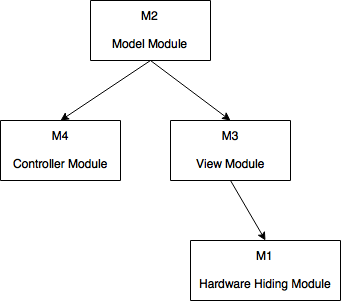
\includegraphics[width=\textwidth]{MGUsesHierarchy.png}
    \caption{Use Hierarchy among Modules}
    \label{FigUH}
\end{figure}

\end{document}